\section{Reconciled computations and negative optimization result}\label{sec:experiments}
\subsection{Evidence selection and elementary controls}
The repository retains both successful and failed campaigns. We reconstructed tables from recorded configurations, per-run outputs and training count traces, rather than from the previous manuscript. A source-hash inventory distinguishes byte-verified outputs, source-snapshot gaps, preserved failed attempts and unattributed copies. Historical driver scripts that overwrite fixed paths were not rerun. The new reconciliation is a deterministic analysis of the archive, not an independent repetition of every optimization trajectory.

An independent exhaustive check of all $64$ simple unweighted four-vertex graphs verifies costs, complementary partitions and exact minima. \Cref{tab:graphs} records representative graphs. Haar averaging gives a uniform law on the $D=\binom{m+k-1}{k}$ Fock compositions, so $\E P_{\CF}=\binom{m}{k}/D$ and $\E\succp=g^*/D$, where $g^*$ is the number of optimal valid \emph{strings}. At $m=4,k=2$, $D=10$. All six balanced strings are optimal on $K_4$, giving $\E\succp=0.6$; $K_{2,2}$ has minimum cut $2$ and four optimal strings, giving $0.4$. A graph-independent Haar success value $0.2$ is therefore incorrect. The Haar baseline is an ensemble average, not a universal per-circuit ceiling~\cite{arkhipov2012}.
\begin{table}[t]
\centering
\begin{tabular}{lrrc}
\hline
Graph & $C^*$ & Optimal strings $g$ & Haar $\mathbb{E}[P_{\rm opt}]$ \\
\hline
Path & 1 & 2 & $\frac{2}{10}$ \\
Cycle & 2 & 4 & $\frac{4}{10}$ \\
$K_4$ & 4 & 6 & $\frac{6}{10}$ \\
$K_{2,2}$ & 2 & 4 & $\frac{4}{10}$ \\
Star & 2 & 6 & $\frac{6}{10}$ \\
\hline
\end{tabular}
\caption{Computed four-vertex, two-photon controls. Balanced bitstrings and their complements are counted separately. The last column is a Haar ensemble expectation, not a trained or measured hardware success rate.}
\label{tab:graphs}
\end{table}


The E01 Haar archive includes size-dependent circuit counts; in particular the $n=10$ sample is smaller than the $n\le8$ samples. It does not provide trained $n=10,12$ optimization evidence. E02 uses the optimal-state mask during optimization and is retained as an oracle-assisted state-preparation diagnostic. E03--E04 compare small-instance objective/optimizer variants, while E06--E09 test structural baselines, spectral information, coherence diagnostics and label sensitivity. None warrants extrapolating a favorable oracle/Haar ratio to an optimum-blind algorithm.

\subsection{Exactly recorded query and attempt budgets}
The primary empirical comparison is E05b. The full grid has $n=4,6,8$, six graph families, two nominal graph seeds, three training seeds and seven method configurations: bosonic and distinguishable meshes, a classical iid multinomial control, a uniform feasible sampler, and classical product-Bernoulli penalty controls at three strengths ($0.1,1,10$). Repeated graph seeds can generate identical graphs; the nominal twelve graph positions at each size contain only $9,9,10$ unique edge lists, respectively. The archived global means retain the nominal grid weighting so the analysis does not select favorable graphs. Intervals use 2000 deterministic percentile bootstrap replicates with the $2.5$th and $97.5$th percentiles: a resampled graph cluster contributes all its optimizer repeats and nominal slots, and the replicate mean is the ratio of their summed probabilities to their record count. These intervals describe this fixed graph grid, rather than a random graph population; resampling seeds as independent graphs would inflate the evidence.

Each optimized trajectory records $120$ objective evaluations, $256$ ideal sampled attempts per evaluation, and a final $4096$-attempt batch: $120\times256+4096=34816$ attempts. This equality does not make classical matrix simulation costs equal to physical circuit shots or to a discrete-search query. Mesh dimension is obtained from its actual coupler list and phases, not equated to the number of Bernoulli parameters. Rejected/colliding outcomes remain in the denominator. For the bosonic, distinguishable and iid multinomial arms, training minimizes the sampled conditional cut plus $2(1-\widehat P_F)$. A batch with no valid outcome receives the fixed value $\sum_E w_{ij}+3$. Penalty arms minimize the sampled full binary QUBO energy. COBYLA uses a 120-call cap, initial radius $0.35$ and tolerance $10^{-7}$; any unspent calls follow a fixed Gaussian local-proposal completion rule of standard deviation $0.1$. Uniform feasible sampling has no trained parameters but spends the same draw budget.

At sizes $n=4,6,8$, the fitted mesh/iid arms train $n(n-1)=12,30,56$ real parameters, with the $n$ input phases fixed because they do not affect fixed-input Fock probabilities. Bernoulli arms train $n=4,6,8$ logits. These dimensions differ. The simulator retains the total non-CF mass as an explicit rejection category, without resolving its internal collision histogram; for $k\ge3$ these unresolved rejection counts do not generally determine the pair moment $M$. In the two-photon bosonic arm, however, every collisional outcome contains one pair and $M=1-P_{\CF}$ exactly. Table~\ref{tab:e05b} and \cref{fig:e05b} show the exact final distribution probabilities after finite-shot training, rather than the noisy success rates in the independent 4096-draw heldout batches. The retrospective optimum is used for evaluation, not the E05b recorded training loss; anti-oracle tests enforce that separation in the recovered public training API.

\begin{table}[t]
\centering\small
\setlength{\tabcolsep}{3pt}
\begin{tabular}{lccc}
\hline
Method & $n=4$ & $n=6$ & $n=8$ \\
\hline
Bosonic & \shortstack{0.652\\{[0.464, 0.804]}} & \shortstack{0.280\\{[0.178, 0.423]}} & \shortstack{0.068\\{[0.033, 0.107]}} \\
Distinguishable & \shortstack{0.713\\{[0.590, 0.835]}} & \shortstack{0.537\\{[0.389, 0.646]}} & \shortstack{0.138\\{[0.075, 0.197]}} \\
Classical iid multinomial & \shortstack{0.421\\{[0.310, 0.532]}} & \shortstack{0.110\\{[0.063, 0.158]}} & \shortstack{0.026\\{[0.016, 0.036]}} \\
Product Bernoulli penalty ($\lambda=0.1$) & \shortstack{0.199\\{[0.135, 0.268]}} & \shortstack{0.057\\{[0.033, 0.089]}} & \shortstack{0.017\\{[0.010, 0.023]}} \\
Product Bernoulli penalty ($\lambda=1$) & \shortstack{0.203\\{[0.141, 0.271]}} & \shortstack{0.056\\{[0.032, 0.088]}} & \shortstack{0.016\\{[0.010, 0.023]}} \\
Product Bernoulli penalty ($\lambda=10$) & \shortstack{0.199\\{[0.127, 0.270]}} & \shortstack{0.056\\{[0.032, 0.092]}} & \shortstack{0.017\\{[0.010, 0.023]}} \\
Uniform feasible & \shortstack{0.528\\{[0.333, 0.718]}} & \shortstack{0.175\\{[0.100, 0.277]}} & \shortstack{0.060\\{[0.036, 0.086]}} \\
\hline
\end{tabular}
\caption{Ideal final success means over 36 runs per method and size, with descriptive graph-cluster percentile intervals. There are 12 nominal graph slots per size but $G=9,9,10$ unique labeled weighted graphs, respectively. Every run uses 120 calls of 256 training draws plus 4096 heldout draws (34816 ideal attempts). Optimizer repeats stay in the same graph cluster; these are not population significance intervals. Each penalty parameter is a separate fully charged run. No hardware shots.}
\label{tab:e05b}
\end{table}

\begin{figure}[tb]
 \centering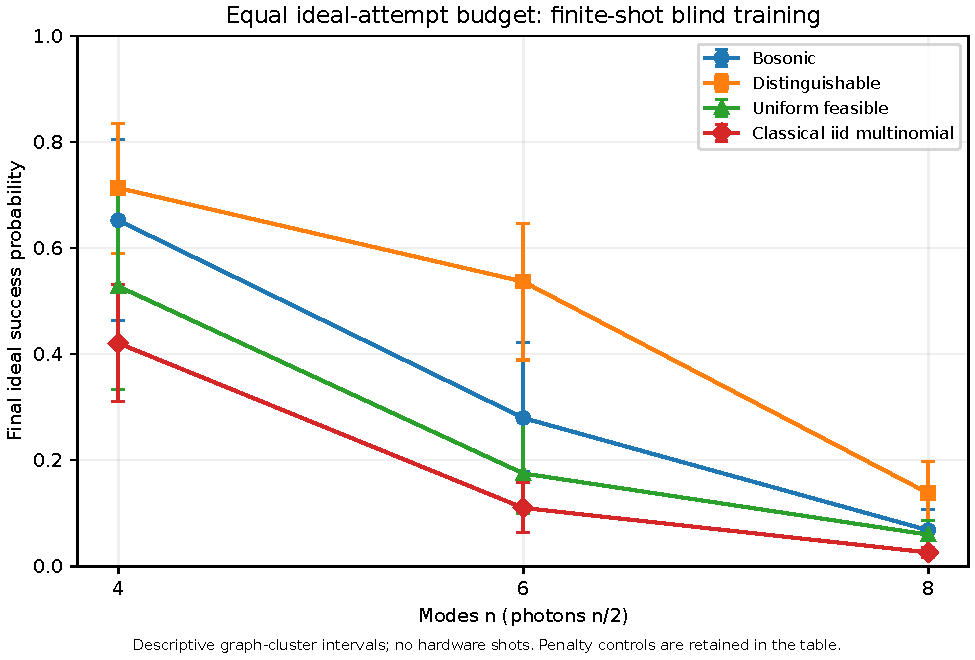
\includegraphics[width=.94\linewidth]{figures/fig_e05b.pdf}
 \caption{Final success of bosonic and distinguishable E05b procedures, with the complete nominal-grid means shown as points. Descriptive intervals resample whole graph clusters, retaining optimizer repeats and nominal-slot multiplicities; they are not a population confidence claim for random graph ensembles. Per-graph and per-seed values, penalty settings and aggregation rules are supplied with the data.}\label{fig:e05b}
\end{figure}

The bosonic final means are lower than the distinguishable means at all three sizes. These observations reject the claimed benefit for this implementation on this grid and budget; they do not prove that every optical optimizer is inferior. Every archived run already encounters an optimal solution during training, so the final circuit probability alone fails to describe problem-solving utility. Count traces locate the first \emph{winning batch}, but do not preserve shot order inside a batch. Exact first-hit shot counts cannot be recovered and are not imputed. Thus a claim of shorter time to first optimum is not supported by these data. A future search trial must save ordered queries and charge preprocessing, restarts, training, final samples and decoding.

The uniform balanced sampler is a relevant feasibility baseline; Bernoulli penalties are a different, weaker control and their three strengths are reported separately. The P21 classical search archive supplies balanced random search, exchange/local improvement and graph-aware controls at a separate cut-query budget. Spectral preprocessing and graph relabeling tests show why a successful optically encoded sample can inherit classically supplied graph structure. These campaigns strengthen the no-benefit assessment, but their differing budgets do not form a matched wall-clock speedup experiment. The new evidence inventory gives their exact provenance and resource units.

ObliQ is an actual hybrid photonic QUBO algorithm~\cite{ranjan2025}, not a synonym for an independent Bernoulli sampler. The authenticated static optical kernel was checked against its archive, Fock calculations and Perceval; literal and physically corrected angle conventions are kept separate. Complete original training, source selection and prefix decoding have not been reproduced, so no end-to-end superiority over authentic ObliQ is claimed.

\subsection{Finite theory checks and retained counterexamples}
The accepted supervised P33 primary/replication data cover all $300$ registered grid circuits, with full-law computations restricted to at most twelve modes; an additional $72$ entries evaluate certificate quantities only. Larger-frame entries evaluate certificate quantities only. Independent complete-law and Perceval controls support implementation consistency within stated tolerances, without proving the theorem. \Cref{fig:density} is generated from those accepted files; unattributed root-level P33 copies are excluded.
\begin{figure}[tb]
 \centering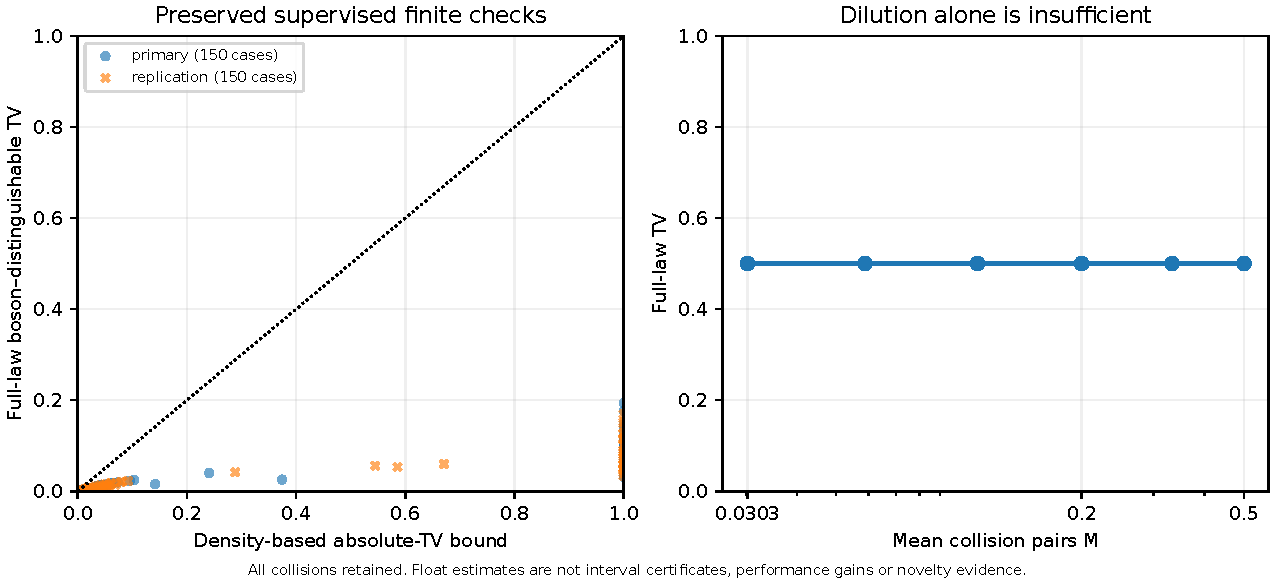
\includegraphics[width=\linewidth]{figures/fig_density.pdf}
 \caption{Left: 300 complete-law grid checks against the coarse density envelope $\Phi(M/c)$ from the accepted supervised primary/replication archive. Right: dilute spectator controls with decreasing collision-pair moment and constant TV. Separate sharp-family and certificate-only large-frame entries are retained in the data; the latter are not full-law comparisons. The sharp family and spectator obstruction test different hypotheses of \cref{thm:density}.}\label{fig:density}
\end{figure}

The P35 low-rank threshold expectation calculation is an exact classical mean-objective control, consistent with known product-state counting methods~\cite{ivanov2020}; it is not a sampler or a new optimization algorithm. Its earlier resource-guard defect and independent post-fix receipt are preserved. A stronger proposed pinched-state curved envelope was refuted in P39 by an exact physical three-photon/nine-mode construction at leakage $18/25$. Its measured output total variation remains below that curve: the refutation concerns the larger auxiliary state metric. The general measured bound $\TV\le\delta$ remains open. Failed searches and nonconverged solvers are retained as such, not promoted into proofs.
